\chapter{K-Means y sus fundamentos}
Los clústeres son la piedra angular del aprendizaje no supervisado. Entre los diferentes algoritmos de agrupación en clústeres, tenemos K-Means.

\section{K-Means}

El algoritmos K-Means particiona los datos en K clústeres distintos, cada uno de ellos representado por la media de los puntos. El objetivo es minimizar la varianza ínter-clúster, haciendo que los grupos tengan datos lo más diferentes posibles entre sí y, al mismo tiempo, asegurar que los elementos dentro de cada grupo sean lo más similares posible entre sí.

\subsection{Diagramas de Voronoi}

Los \textbf{diagramas de Voronoi} o \textbf{polígonos de Thiessen} son una forma de dividir el espacio en regiones basadas en la proximidad a un conjunto específico de puntos. Cada región en el diagrama de Voronoi está asociado a uno de estos sitios y contiene todos los puntos del espacio que están mas cerca de ese sitio que de cualquier otro.

En ciencia de datos, estos diagramas se utilizan para ilustrar cómo se agrupan los datos en torno a los centroides; en K-Means, cada región de Voronoi se corresponde a un clúster generado por el algoritmo.

Las características clave son:

\begin{itemize}
    \item Cada región está delimitada por las líneas bisectrices.

    \item Los vértices de los polígonos de Voronoi están ubicados en puntos donde tres o más sitios se encuentran equidistantes.

    \item Pueden ser bidimensionales o tridimensionales.
\end{itemize}


\subsection{El algoritmo K-Means: Paso a paso}

\begin{enumerate}
    \item Preprocesamiento de los datos: para mejorar la calidad y precisión de los modelos.

    \item Inicialización de centroides: se comienza el ciclo seleccionando aleatoriamente K puntos como centroides iniciales; los centroides son puntos que representan el centro de cada uno de los K grupos que se quieren identificar.

    \item Asignación de puntos a centroides: para cada punto del dataset, se calcula la distancia entre ese punto y cada uno de los centroides; luego, se asigna el punto al centroide más cercano.

    \item Actualización de los centroides: después de asignar cada punto a un centroide, se recalcula la posición de cada centroide como el centroide del grupo de puntos asignados a él: el nuevo centroide es el promedio de todas las coordenadas de los puntos asignados al grupo.

    \item Repetición: los dos pasos anteriores se repiten iterativamente hasta que los centroides dejen de cambiar de manera significativa o hasta que se alcance un número máximo de iteraciones.

    \item Convergencia: cuando los centroides permanecen constantes entre iteraciones y los puntos están asignados a los grupos de manera estable, hemos llegado a una situación de convergencia.

    \item Resultado final: tenemos un conjunto de K grupos, donde cada grupo está representado por su centroide.
\end{enumerate}


\section{Elección del número de clústeres}
Uno de los principales desafíos de los problemas de agrupamiento reside en elegir el número de grupos que representan al conjunto de datos. 

Un número de grupos erróneo implica que se tendrán grupos que no representan al conjunto de datos. Si conocemos el dominio de los datos, la tarea es más sencilla, pero no siempre es el caso.

Los dos principios básicos para encontrar el número óptimo de clústeres son:

\begin{itemize}
    \item Los puntos dentro del grupo deben ser lo más similares posible.

    \item Los puntos que pertenecen a distintos grupos deben ser lo más distintos posible.
\end{itemize}

Con esto en mente, vemos dos métricas que se utilizarán para hallar el número ideal de clústeres.

\subsection{Métricas}
\subsubsection{Inercia}

\begin{definition}
    La \textbf{inercia} se calcula como la suma de las distancias al cuadrado entre los puntos de datos y los centros de los grupos a los qu pertenece:

    \begin{equation}
        I=\sum_{i=1}^n\norm{x_i-\mu_{c(i)}}^2,
    \end{equation}

    donde: $n$ es el número total de puntos, $x_i$ es el i-ésimo punto de datos, $\mu_{c(i)}$ es el centroide del clúster al que pertenece el punto $x_i$ y $\norm{x_i-\mu_{c(i)}}^2$ es la distancia euclidiana entre el punto $x_i$ y su centroide correspondiente $\mu_{c(i)}$.
\end{definition}

\subsubsection{El método del codo}
\begin{definition}
    El \textbf{método del codo} consiste en trazar la inercia en función del número de  clústeres y observar el punto en el que la inercia comienza a desacelerarse, formando un codo. Este método es útil para indicarnos que el valor óptimo para $K$ es el punto donde comienza a formarse el codo.
\end{definition}

\begin{figure}[ht]
    \centering
    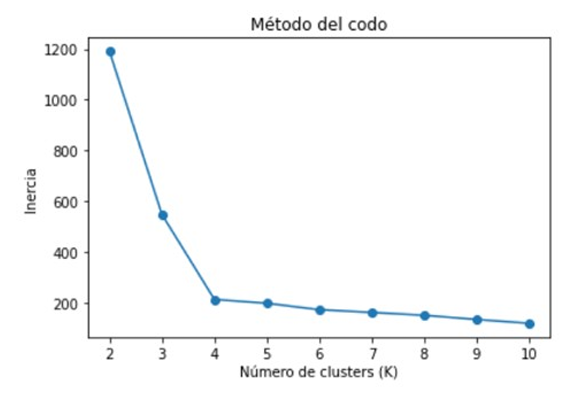
\includegraphics[width=0.85\linewidth]{imagenes/metodo-codo.png}
    \label{fig:metodo-codo}
\end{figure}

Sin embargo, este método puede ser muy subjetivo.

\subsubsection{El coeficiente de la silueta}
\begin{definition}
    El coeficiente de la silueta nos muestra un resumen de la variación dentro de un grupo y la variación entre grupos. Para cada observación, se calcula la distancia al centroide del grupo al que pertenece y lo denominamos $a$. Además, calculamos la distancia al segundo mejor centroide del grupo más cercano que no es el suyo y lo denominamos $b$. Aplicamos la siguiente fórmula:

    \begin{equation*}
        s=\dfrac{b-a}{\max(a,b)}
    \end{equation*}
\end{definition}


En un escenario ideal, la distancia $a$ es muy pequeña en comparación con la distancia $b$ por lo que el valor de $s$ es cercano a $1$; si la distancia $a$ y $b$ son similares, entonces $s$ tiende a $0$. Si la agrupación es mala, $a\ge b$ y $s$ es negativo o cercano a $-1$.

Utilizando el coeficiente de la silueta, se utiliza el método de la silueta para hallar el valor óptimo de $k$:

\begin{enumerate}
    \item Se calcula la puntuación de la silueta para cada punto del conjunto de datos.

    \item Se promedian los puntos para cada grupo.

    \item Se trazan las puntuaciones promedios para diferentes valores de $k$.

    \item El valor óptimo para $k$ es aquel en el que la puntuación de la silueta es el promedio más alto.
\end{enumerate}

\begin{figure}[ht]
    \centering
    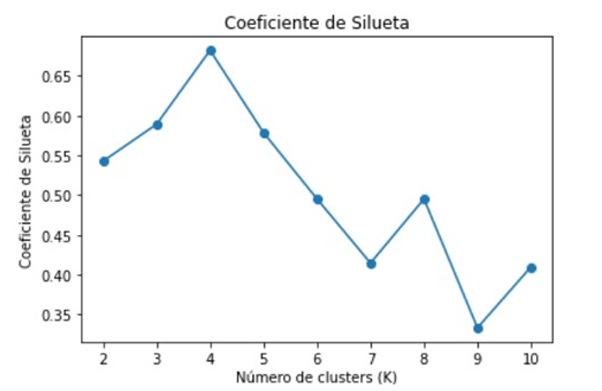
\includegraphics[width=0.85\linewidth]{imagenes/coeficiente-silueta.png}
    \label{fig:coeficiente-silueta}
\end{figure}

\subsubsection{Estadística de la brecha}

Para evaluar la calidad de los clústeres generados por K-Means, utilizamos la media de la estadística de la brecha. Esta métrica compara la inercia intra-clúster de un conjunto de datos con la que se esperaría encontrar en un conjunto de datos aleatorios sin estructura de clustering, con la inercia de los clústeres generados con los datos originales

\begin{enumerate}
    \item  \textbf{Dispersión intra-clúster con datos originales}: primero se calcula la inercia intra-clúster de los datos originales utilizando el algoritmo K-Means para diferentes valores de k. Este valor mide cuán compactos y cohesivos son los clústeres formados por el algoritmo para cada valor de k.

    \item \textbf{Dispersión intra-clúster con datos aleatorios}: se generan varios conjuntos de datos de referencia aleatorios (también conocidos como conjuntos de datos nulos)  manteniendo la estructura de los datos originales, pero mezclando aleatoriamente  las etiquetas de los puntos. Para cada conjunto de datos de referencia se calcula la  inercia intra-clúster utilizando K-Means.

    \item  \textbf{Cálculo de la brecha}: la brecha se calcula como la diferencia entre la inercia intra-clúster esperada en los datos aleatorios y la inercia intra-clúster observada en los datos originales. Se promedia esta diferencia sobre todos los conjuntos de datos de  referencia.

    \item \textbf{Selección del número óptimo de clústeres}: el número óptimo de clústeres se  elige el valor de K que maximiza la brecha. En otras palabras, se busca el punto donde la dispersión intra-clúster observada en los datos reales es menor que la dispersión de los datos aleatorios.
\end{enumerate}


\begin{figure}[ht]
    \centering
    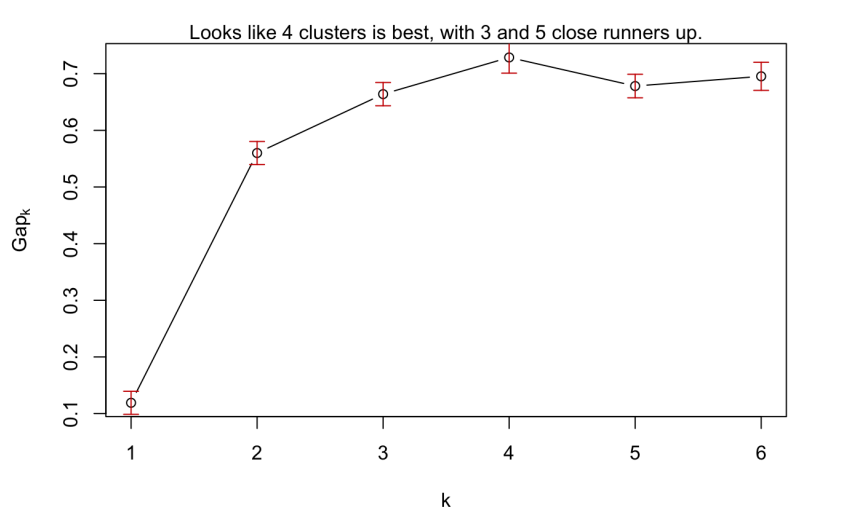
\includegraphics[width=0.85\linewidth]{imagenes/estadística-brecha.png}
    \label{fig:estadistica-brecha}
\end{figure}

\section{Ventajas y desventajas de K-Means}

\begin{table}[ht]
  \centering
  \begin{tabular}{|c|c|}
    \hline
    Ventajas de K-Means & Desventajas de K-Means \\ \hline
    Popular &  Definir el número óptimo de clústeres.\\ \hline
    Sencillo de aplicar & Sensible a \textit{outliers} \\ \hline
    Eficiencia computacional &  \\ \hline
    Puede manejar datos de alta dimensionalidad &  \\ \hline
    Escalable &  \\ \hline
    Flexible &  \\ \hline
    Fácil interpretabilidad &  \\ \hline
  \end{tabular}
  \label{tab:ventajas_desventajas-K-Means}
\end{table}